% Options for packages loaded elsewhere
\PassOptionsToPackage{unicode}{hyperref}
\PassOptionsToPackage{hyphens}{url}
\PassOptionsToPackage{dvipsnames,svgnames,x11names}{xcolor}
%
\documentclass[
  10pt,
]{article}
\usepackage{amsmath,amssymb}
\usepackage{iftex}
\ifPDFTeX
  \usepackage[T1]{fontenc}
  \usepackage[utf8]{inputenc}
  \usepackage{textcomp} % provide euro and other symbols
\else % if luatex or xetex
  \usepackage{unicode-math} % this also loads fontspec
  \defaultfontfeatures{Scale=MatchLowercase}
  \defaultfontfeatures[\rmfamily]{Ligatures=TeX,Scale=1}
\fi
\usepackage{lmodern}
\ifPDFTeX\else
  % xetex/luatex font selection
\fi
% Use upquote if available, for straight quotes in verbatim environments
\IfFileExists{upquote.sty}{\usepackage{upquote}}{}
\IfFileExists{microtype.sty}{% use microtype if available
  \usepackage[]{microtype}
  \UseMicrotypeSet[protrusion]{basicmath} % disable protrusion for tt fonts
}{}
\makeatletter
\@ifundefined{KOMAClassName}{% if non-KOMA class
  \IfFileExists{parskip.sty}{%
    \usepackage{parskip}
  }{% else
    \setlength{\parindent}{0pt}
    \setlength{\parskip}{6pt plus 2pt minus 1pt}}
}{% if KOMA class
  \KOMAoptions{parskip=half}}
\makeatother
\usepackage{xcolor}
\usepackage[top=1in, bottom=1in, left=1in, right=1in]{geometry}
\usepackage{longtable,booktabs,array}
\usepackage{calc} % for calculating minipage widths
% Correct order of tables after \paragraph or \subparagraph
\usepackage{etoolbox}
\makeatletter
\patchcmd\longtable{\par}{\if@noskipsec\mbox{}\fi\par}{}{}
\makeatother
% Allow footnotes in longtable head/foot
\IfFileExists{footnotehyper.sty}{\usepackage{footnotehyper}}{\usepackage{footnote}}
\makesavenoteenv{longtable}
\usepackage{graphicx}
\makeatletter
\newsavebox\pandoc@box
\newcommand*\pandocbounded[1]{% scales image to fit in text height/width
  \sbox\pandoc@box{#1}%
  \Gscale@div\@tempa{\textheight}{\dimexpr\ht\pandoc@box+\dp\pandoc@box\relax}%
  \Gscale@div\@tempb{\linewidth}{\wd\pandoc@box}%
  \ifdim\@tempb\p@<\@tempa\p@\let\@tempa\@tempb\fi% select the smaller of both
  \ifdim\@tempa\p@<\p@\scalebox{\@tempa}{\usebox\pandoc@box}%
  \else\usebox{\pandoc@box}%
  \fi%
}
% Set default figure placement to htbp
\def\fps@figure{htbp}
\makeatother
\setlength{\emergencystretch}{3em} % prevent overfull lines
\providecommand{\tightlist}{%
  \setlength{\itemsep}{0pt}\setlength{\parskip}{0pt}}
\setcounter{secnumdepth}{5}
% definitions for citeproc citations
\NewDocumentCommand\citeproctext{}{}
\NewDocumentCommand\citeproc{mm}{%
  \begingroup\def\citeproctext{#2}\cite{#1}\endgroup}
\makeatletter
 % allow citations to break across lines
 \let\@cite@ofmt\@firstofone
 % avoid brackets around text for \cite:
 \def\@biblabel#1{}
 \def\@cite#1#2{{#1\if@tempswa , #2\fi}}
\makeatother
\newlength{\cslhangindent}
\setlength{\cslhangindent}{1.5em}
\newlength{\csllabelwidth}
\setlength{\csllabelwidth}{3em}
\newenvironment{CSLReferences}[2] % #1 hanging-indent, #2 entry-spacing
 {\begin{list}{}{%
  \setlength{\itemindent}{0pt}
  \setlength{\leftmargin}{0pt}
  \setlength{\parsep}{0pt}
  % turn on hanging indent if param 1 is 1
  \ifodd #1
   \setlength{\leftmargin}{\cslhangindent}
   \setlength{\itemindent}{-1\cslhangindent}
  \fi
  % set entry spacing
  \setlength{\itemsep}{#2\baselineskip}}}
 {\end{list}}
\usepackage{calc}
\newcommand{\CSLBlock}[1]{\hfill\break\parbox[t]{\linewidth}{\strut\ignorespaces#1\strut}}
\newcommand{\CSLLeftMargin}[1]{\parbox[t]{\csllabelwidth}{\strut#1\strut}}
\newcommand{\CSLRightInline}[1]{\parbox[t]{\linewidth - \csllabelwidth}{\strut#1\strut}}
\newcommand{\CSLIndent}[1]{\hspace{\cslhangindent}#1}
\usepackage{xcolor}
\usepackage{hyperref}
\hypersetup{colorlinks=true, linkcolor=blue, urlcolor=blue, citecolor=blue}
\usepackage{float}
\usepackage{booktabs}
\usepackage{caption}
\usepackage{enumitem}
\usepackage{fancyhdr}
\usepackage{lastpage}
\usepackage{microtype}
\usepackage{titlesec}
\usepackage{fvextra}
\setcounter{secnumdepth}{0}
\floatplacement{figure}{H}
\floatplacement{table}{H}
\captionsetup{font=footnotesize, labelfont=bf}
\setlength{\parindent}{0pt}
\setlength{\parskip}{0.2em}
\setlist{nosep,leftmargin=*}
\titlespacing*{\section}{0pt}{0.58em}{0.2em}
\titlespacing*{\subsection}{0pt}{0.48em}{0.18em}
\titleformat{\section}{\large\bfseries}{\thesection}{0.5em}{}
\titleformat{\subsection}{\normalsize\bfseries}{\thesubsection}{0.5em}{}
\makeatletter
\renewcommand{\maketitle}{}
\makeatother
\fancypagestyle{plain}{
  \fancyhf{}
  \renewcommand{\headrulewidth}{0pt}
  \renewcommand{\footrulewidth}{0pt}
  \fancyfoot[C]{\small Page~\thepage~of~\pageref{LastPage}}
}
\pagestyle{fancy}
\fancyhf{}
\setlength{\headheight}{13pt}
\fancyhead[L]{\small Saijo, Roop, and Shoaib}
\fancyhead[R]{\small NFL WR Contract Projection}
\fancyfoot[C]{\small Page~\thepage~of~\pageref{LastPage}}
\renewcommand{\headrulewidth}{0.35pt}
\renewcommand{\footrulewidth}{0.35pt}
\sloppy
\usepackage{booktabs}
\usepackage{longtable}
\usepackage{array}
\usepackage{multirow}
\usepackage{wrapfig}
\usepackage{float}
\usepackage{colortbl}
\usepackage{pdflscape}
\usepackage{tabu}
\usepackage{threeparttable}
\usepackage{threeparttablex}
\usepackage[normalem]{ulem}
\usepackage{makecell}
\usepackage{xcolor}
\usepackage{bookmark}
\IfFileExists{xurl.sty}{\usepackage{xurl}}{} % add URL line breaks if available
\urlstyle{same}
\hypersetup{
  pdftitle={Projecting NFL Wide Receiver Contracts},
  pdfauthor={Rento Saijo, Atticus Roop, and Manahil Shoaib},
  colorlinks=true,
  linkcolor={blue},
  filecolor={Maroon},
  citecolor={blue},
  urlcolor={blue},
  pdfcreator={LaTeX via pandoc}}

\title{Projecting NFL Wide Receiver Contracts}
\usepackage{etoolbox}
\makeatletter
\providecommand{\subtitle}[1]{% add subtitle to \maketitle
  \apptocmd{\@title}{\par {\large #1 \par}}{}{}
}
\makeatother
\subtitle{Term Probabilities and Cap-Share Price for the 2026 Veteran Market}
\author{Rento Saijo, Atticus Roop, and Manahil Shoaib}
\date{May 11, 2026}

\begin{document}
\maketitle

\begin{titlepage}
\thispagestyle{empty}
\begin{center}
\vspace*{0.72in}
{\LARGE\bfseries Projecting NFL Wide Receiver Contracts\par}
\vspace{0.20in}
{\large Term Probabilities and Cap-Share Price for the 2026 Veteran Market\par}
\vspace{0.32in}
{\normalsize Rento Saijo, Atticus Roop, and Manahil Shoaib\par}
\vspace{0.12in}
{\normalsize May 11, 2026\par}
\end{center}
\vspace{0.35in}
\begin{center}
\begin{minipage}{0.78\textwidth}
\small
\textbf{Abstract.} This paper asks whether public data can predict three parts of the veteran NFL wide receiver contract market: contract term, average annual value as a salary-cap share (AAV\%), and the variables that make those forecasts credible. The project begins with Spotrac wide receiver contract exports, then enriches each deal with nflverse player identity, rosters, combine measurements, receiving production, snap usage, Next Gen receiving metrics, team context, schedule timing, and ESPN transaction dates when matched. The football problem motivates the modeling design: term measures how much commitment a team is willing to make, while AAV\% measures annual price. We therefore fit a multiclass term model and a conditional AAV\% model. Tuned XGBoost performs best on signed 2026 validation contracts, with term log loss 0.537 and AAV\% RMSE 0.0057. Scoring 163 unsigned 2026 receivers produces a short-term market: every player has a modal one-year deal, with median expected AAV of \$1.11M. The accompanying dashboard (\href{https://rentosaijo.github.io/NFLxC/}{rentosaijo.github.io/NFLxC}) translates those forecasts into player-level term-price menus for roster and salary-cap planning. The conclusion is predictive rather than causal: public data can separate likely term scenarios from price scenarios, but guarantees, injuries, team needs, and private negotiations remain outside the observed data.
\end{minipage}
\end{center}
\end{titlepage}
\setcounter{page}{1}

\section{Introduction and Background}\label{introduction-and-background}

The wide receiver market looks simple only from a distance. A receiver's most visible work is in the passing game: running routes, creating separation, catching the ball, gaining yards after the catch, and forcing defenses to account for him. Yet the same position label covers several labor-market roles. One player may be an offense's first option, another may be a field-stretcher or slot specialist, and a third may be valued for injury depth, package rotation, or special teams. When a team signs a receiver, it is not just buying last year's catches. It is deciding how much roster space, cap space, and future risk to attach to a particular role.

That decision has two pieces that should not be collapsed into one dollar figure. The NFL salary cap is a league-wide annual spending limit, so the same raw salary can mean different things in different years. Average annual value (AAV) reports dollars per contract year, while AAV\% divides AAV by the salary cap at signing and puts deals from different eras on the same economic scale. Contract term measures a different kind of value: commitment. A one-year deal preserves flexibility; a multi-year deal usually signals stronger leverage, a stable projected role, or confidence that the player will remain useful beyond the next season. Two receivers can be paid similarly per year while receiving very different levels of security.

This paper asks three linked predictive questions. Can public information available before signing forecast the term of a veteran wide receiver contract? Conditional on a possible term, can it forecast the player's annual price as a share of the cap? Which signals make those forecasts credible: production, age, prior contracts, team context, market timing, usage, or tracking-based receiving metrics? The modeling design follows the football problem. Instead of producing one contract estimate, the project builds a term classifier over one, two, three, four, and five+, then pairs it with a conditional AAV\% model that prices each term scenario.

\section{Data, EDA, and Methods}\label{data-eda-and-methods}

The data pipeline starts with Spotrac wide receiver contract exports by decade (\citeproc{ref-spotrac}{Spotrac 2026}), which provide the contract spine: player, team, start and end years, term, value, AAV, and AAV\%. The analysis keeps veteran, non-entry wide receiver deals because rookie contracts are heavily shaped by draft slot and league bargaining rules, while veteran contracts more directly reveal how teams price a player in the open market. Cleaning turns those public records into a pre-signing modeling file by standardizing names and teams, parsing contract economics, converting AAV\% to cap share, repairing inconsistent end years, removing yearly rows already embedded inside earlier multi-year contracts, and building previous-contract features. The workflow then attaches nflverse player references, rosters, combine measurements, receiving statistics, snap counts, Next Gen receiving metrics, team offense, and schedules (\citeproc{ref-nflreadr}{nflverse 2026}). Snap counts describe playing-time usage; Next Gen receiving metrics use player-tracking data to describe how a receiver creates and performs on targets. ESPN transaction descriptions supply signing dates when a reliable match is available; otherwise the workflow uses an explicit March 15 offseason proxy.

\begin{table}[H]
\centering
\caption{\label{tab:main-split-table}\label{tab:main-splits} Modeling files and their roles in the analysis.}
\centering
\resizebox{\ifdim\width>\linewidth\linewidth\else\width\fi}{!}{
\fontsize{6.9}{8.9}\selectfont
\begin{tabular}[t]{lrrc>{\raggedright\arraybackslash}p{3.1in}}
\toprule
Split & Rows & Players & Years & Use in Paper\\
\midrule
Train & 2,796 & 1,305 & 2002-2025 & Historical signed veteran WR contracts used to learn the relationship between pre-signing information and contract outcomes.\\
Validate & 91 & 91 & 2026 & Signed 2026 contracts held out for model comparison, so performance is checked on newer market behavior.\\
Test & 163 & 163 & 2026 & Unsigned 2026 free agents scored by the final models; outcomes are intentionally unknown at prediction time.\\
\bottomrule
\end{tabular}}
\end{table}

Table \ref{tab:main-splits} shows the final row universe and the role of each split. Because each row is a contract rather than a unique player, some receivers appear more than once across their careers. That structure captures how players move through market stages, but it also creates dependence if one player's rows are split randomly across resamples. To reduce repeated-player leakage, all model tuning uses player-grouped folds instead of the typical random \texttt{k}-fold. Lasso and ridge coefficients are treated as predictive audit signals rather than independent causal effects. Tree-based models do not rely on linear-model error independence for coefficient tests, but they can still look too strong if one player's contracts leak across folds. Prior-season predictors also respect time order: they use the two most recent completed regular seasons before the signing reference date, with the most recent season weighted twice as heavily.

\begin{figure}[H]

{\centering 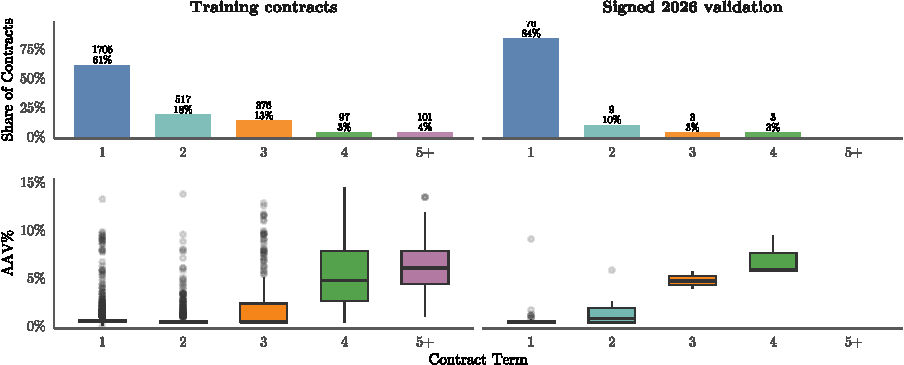
\includegraphics[width=\linewidth]{paper_files/figure-latex/eda-term-price-plot-1} 

}

\caption{\label{fig:eda-term-price} Term concentration and term-price separation in the labeled data. Bars show each term class as a share of contracts; boxes show AAV\% within each term. The validation market is more one-year concentrated than training, while longer deals occupy higher cap-share ranges, motivating probability-based term evaluation and a conditional AAV\% model.}\label{fig:eda-term-price-plot}
\end{figure}

The exploratory pattern in Figure \ref{fig:eda-term-price} explains why the project separates commitment from price. One-year deals are common in training (61.0\%) and even more dominant in signed 2026 validation contracts (83.5\%). In that setting, raw accuracy can reward a model for saying ``one year'' too often, so term is better evaluated as a probability distribution across possible commitments. AAV\% has a different shape: longer deals tend to occupy higher cap-share ranges, but the boxes still overlap enough to show that annual price is not just a disguised term label. The same receiver can have a high-probability one-year scenario and a lower-probability multi-year scenario with a different annual price, which is the negotiation surface the two-model design represents.

Once the data are organized around the signing date, the modeling workflow uses \texttt{tidymodels} recipes and engines (\citeproc{ref-tidymodels}{tidymodels 2026}) to keep preprocessing consistent across candidates. Identifiers, audit dates, signing team labels, and current-contract outcomes are removed before fitting. Categorical predictors receive unknown/novel handling, mode imputation, and dummy encoding; numeric predictors receive median imputation, zero-variance filtering, and normalization. The term task drops current AAV and AAV\% to avoid direct leakage. The AAV\% task drops current AAV but keeps term because the final scorer asks what the player's cap-share price would be under supplied one-year, two-year, three-year, four-year, and five-or-more-year scenarios. Screening compared null, linear, penalized, tree, random forest, boosted, neural-network, and LightGBM-style candidates where available, then final tuning used Bayesian optimization with grouped five-fold cross-validation by player. The term model minimizes multinomial log loss; the AAV\% model minimizes RMSE. XGBoost is selected for both predictive tasks (\citeproc{ref-xgboost}{Chen and Guestrin 2016}), while lasso multinomial regression and ridge regression are retained as audit models (\citeproc{ref-glmnet}{Friedman, Hastie, and Tibshirani 2010}).

\section{Results and Discussion}\label{results-and-discussion}

The validation results are easiest to read against the imbalance found in EDA. On the signed 2026 contracts, the tuned XGBoost term model achieved log loss 0.537, Brier score 0.057, and accuracy 82.4\%. The null majority classifier has higher raw accuracy because 76 of 91 validation contracts are one-year deals, but it assigns weaker probabilities. That is not a contradiction; it is the central evaluation problem. Accuracy asks whether the top guess was right, while log loss and Brier score ask whether the model distributed its confidence sensibly across all possible lengths. For roster planning, the useful output is a probability profile. The XGBoost AAV\% model achieved RMSE 0.0057, MAE 0.0026, and \(R^2 = 0.903\). At the implied 2026 cap, that RMSE is roughly \$1.71M, accurate enough for market screening while leaving room for private information that public data cannot observe.

\begin{table}[H]
\centering
\caption{\label{tab:main-results-table}\label{tab:main-results} Main validation evidence and how it should be read.}
\centering
\resizebox{\ifdim\width>\linewidth\linewidth\else\width\fi}{!}{
\fontsize{6.7}{8.7}\selectfont
\begin{tabular}[t]{ll>{\raggedright\arraybackslash}p{1.75in}>{\raggedright\arraybackslash}p{2.35in}}
\toprule
Question & Model or Benchmark & Validation Evidence & Interpretation\\
\midrule
Contract term & Tuned XGBoost & Log loss 0.537; Brier 0.057; accuracy 82.4\% & Useful for ranking likely term scenarios rather than declaring one certain answer.\\
Contract term benchmark & Null majority & Accuracy 83.5\%, but weaker probability scores & Shows why raw accuracy is misleading in a one-year-heavy market.\\
AAV\% conditional on term & Tuned XGBoost & RMSE 0.0057; MAE 0.0026; R-squared 0.903 & Useful for translating player, role, market, and term information into cap-share price.\\
\bottomrule
\end{tabular}}
\end{table}

The tuned comparisons in Appendix B explain why the final system keeps both predictive and audit models. XGBoost is the best validation choice for term by log loss and for AAV\% by RMSE, but the margins over random forest and ridge-style alternatives are small enough that interpretability still matters. The lasso term model and ridge AAV\% model check whether the stronger nonlinear models are leaning on football-plausible information instead of hidden artifacts, especially in a term task where predicting one year for nearly everyone can look deceptively successful.

The interpretation artifacts in Appendix C tell a coherent contract story. Term importance is led by contract number, years of experience, previous-team and matching indicators, prior timing, age, and previous market value; recent production appears, but it is not the dominant family. Compensation importance shifts toward weighted receiving yards, yards per game, first downs per game, target share, prior cap share, snap role, and the supplied term scenario. That split matches the way a front office might separate questions internally: term is mainly a commitment and career-stage problem, while AAV\% is more directly a receiving-value and market-price problem.

When applied to the unsigned 2026 receiver pool, the forecasts describe a short-term market with meaningful price variation inside it. All 163 scored players have a modal one-year contract, the mean one-year probability is 85.8\%, and the mean probability of any multi-year outcome is 14.2\%. That does not make the players interchangeable; it says that, by this point in the offseason, the remaining unsigned market is mostly made up of receivers whom teams may value for immediate roles without wanting a long commitment. Price remains right-skewed, with mean expected AAV of \$1.49M, median expected AAV of \$1.11M, and a maximum of \$11.52M. Deebo Samuel, Jauan Jennings, and Keenan Allen top the expected-AAV ranking, but even their modal forecast remains one year. A general manager can use the term-price menu to compare one-year depth options, higher-cost starter candidates, and rare multi-year possibilities while keeping the team's total cap plan coherent. Player-level menus are available in the \href{https://rentosaijo.github.io/NFLxC/}{companion dashboard}, and Appendix D shows both the market board and scenario paths.

The broader conclusion is that the project is strongest as a structured way to separate contract questions that are often blended together. Term is predictable enough to rank probabilities, though the validation distribution makes hard class labels too blunt. AAV\% is meaningfully predictable when the model is given a term scenario. Contract history and career stage explain commitment; receiving production, prior price, role, and term explain compensation. Framed as an actionable front-office insight, the model helps identify which receivers are plausibly short-term cap-efficient pieces and which require a larger annual allocation, while the dashboard turns that comparison into a player-by-player planning board.

\section{Limitations and Future Work}\label{limitations-and-future-work}

The main limitations come from measurement, validation size, and generalizability. Public contract data do not fully observe guarantees, incentives, option years, injuries, cap room, depth-chart need, agent leverage, or competing offers, so two deals with the same term and AAV\% can carry very different economic risk. Signing-date matches cover only part of history, player identity matching is probabilistic for some fringe players, and Next Gen receiving coverage is thin before recent seasons. The validation set is also small: only 91 signed 2026 contracts, heavily concentrated in one-year deals. That market shape is informative, but it means small metric differences and rare multi-year predictions should be read as screening evidence rather than precise estimates.

Future work should add guarantees and incentives as outcomes, automate market refreshes, report calibration and prediction intervals, and test the model across repeated free-agent cycles. The most useful extension would be team-player matching with cap space, receiver depth chart, offensive style, quarterback quality, and target vacancy, because a receiver's likely price and term can change with the destination.

\newpage

\section{Appendix}\label{appendix}

\subsection{Appendix A: Data Construction and Feature Coverage}\label{appendix-a-data-construction-and-feature-coverage}

\begin{table}[H]
\centering
\caption{\label{tab:data-sources-table}\label{tab:data-sources} Data sources and how each source enters the project.}
\centering
\resizebox{\ifdim\width>\linewidth\linewidth\else\width\fi}{!}{
\fontsize{7.3}{9.3}\selectfont
\begin{tabular}[t]{>{\raggedright\arraybackslash}p{1.55in}>{\raggedright\arraybackslash}p{4.1in}}
\toprule
Source & Role in Project\\
\midrule
Spotrac WR contract exports & Contract spine: player, team, start/end years, term, value, AAV, AAV\%, age, guarantees/bonuses for parsing.\\
nflreadr player, roster, combine, stats, snap, NGS, team, and schedule data & Public pre-signing player identity, athletic profile, production, usage, receiver-tracking, team offense, and season-calendar context.\\
ESPN NFL transactions API & Observed or likely signing dates used to reduce temporal leakage in prior-season feature windows.\\
Derived market context & Rolling veteran WR market anchors from prior local contract records: count, median term, AAV, AAV\%, p75 AAV\%, and signing age.\\
\bottomrule
\end{tabular}}
\end{table}

The reproducible data workflow begins with three local Spotrac wide receiver contract exports covering the 2000s, 2010s, and 2020s. Table \ref{tab:data-sources} documents the provenance of each data family. The local contract files define the target rows; the external sources add information that would plausibly be known before signing. The project repository is available at \href{https://github.com/RentoSaijo/NFLxC}{github.com/RentoSaijo/NFLxC}; it contains the cleaning, model-fitting, validation, scoring, paper, and dashboard workflow needed to rebuild the analysis from the source exports and public data pulls.

\begin{table}[H]
\centering
\caption{\label{tab:response-table}\label{tab:responses} Modeled responses and statistical rationale.}
\centering
\resizebox{\ifdim\width>\linewidth\linewidth\else\width\fi}{!}{
\fontsize{7.1}{9.1}\selectfont
\begin{tabular}[t]{l>{\raggedright\arraybackslash}p{2.25in}>{\raggedright\arraybackslash}p{2.45in}}
\toprule
Response & Definition & Why This Target\\
\midrule
term & Reported contract length in years; deals of five or more years are grouped into the 5+ class. & Represents team commitment and player leverage; treated as a probability distribution because one-year deals dominate the validation market.\\
aavPerc & Average annual value divided by league salary cap at signing, modeled as a decimal share. & Normalizes dollars across eras and gives a price target that can be translated back to 2026 dollars.\\
\bottomrule
\end{tabular}}
\end{table}

Table \ref{tab:responses} defines the two modeled responses. This distinction is the reason the final workflow has two model sets: term is a commitment outcome, while AAV\% is a price outcome evaluated under a supplied term scenario.

\begin{table}[H]
\centering
\caption{\label{tab:data-splits-table}\label{tab:data-splits} Modeling data after cleaning.}
\centering
\resizebox{\ifdim\width>\linewidth\linewidth\else\width\fi}{!}{
\fontsize{7.5}{9.5}\selectfont
\begin{tabular}[t]{l>{\raggedright\arraybackslash}p{2.95in}rrc}
\toprule
Split & Role & Rows & Players & Years\\
\midrule
Train & Signed veteran WR contracts used for fitting and tuning & 2,796 & 1,305 & 2002-2025\\
Validate & Signed 2026 veteran WR contracts used for held-out evaluation & 91 & 91 & 2026\\
Test & Unsigned 2026 WR free agents scored by the final models & 163 & 163 & 2026\\
\bottomrule
\end{tabular}}
\end{table}

Table \ref{tab:data-splits} gives the final row universe after cleaning. The split is time-based rather than random because the intended use case is forward projection into an unsigned free-agent market.

\begin{table}[H]
\centering
\caption{\label{tab:cleaning-table}\label{tab:cleaning} Key cleaning and temporal-logic decisions.}
\centering
\resizebox{\ifdim\width>\linewidth\linewidth\else\width\fi}{!}{
\fontsize{7.1}{9.1}\selectfont
\begin{tabular}[t]{l>{\raggedright\arraybackslash}p{4.7in}}
\toprule
Step & Implementation Detail\\
\midrule
Contract parsing & Row-bind WR contract files, standardize names/teams, parse numeric economics, convert AAV\% to cap share, and repair inconsistent end years with startYear + term - 1.\\
Embedded-row removal & Drop yearly rows already covered by an earlier multi-year deal for the same player/team before building contract-history variables.\\
Entry-like filtering & Exclude contracts at rookieSeason or first observed contracts with ageAtSigning <= 23 to avoid mixing rookie-scale economics with veteran pricing.\\
Player matching & Join normalized contract names to nflverse player references, then prefer candidates by signing-age gap, rookie-season plausibility, roster backfill, and position context.\\
Signing-date reference & Use matched ESPN transaction dates when available; otherwise use an explicit March 15 offseason proxy for the contract start year.\\
Prior-season windows & Use the two most recent fully completed regular seasons before the reference date, not a mechanical startYear - 1 / startYear - 2 rule.\\
Missing-data policy & Keep raw missing season fields as NA, collapse weighted values to the observed season when only one year exists, set missing deltas to 0, and retain availability flags.\\
\bottomrule
\end{tabular}}
\end{table}

Table \ref{tab:cleaning} summarizes the cleaning decisions that make the rows reproducible and reduce leakage. The most important details are the removal of entry-like contracts, the removal of embedded rows already covered by prior multi-year deals, and the use of signing-date-aware prior seasons.

\begin{table}[H]
\centering
\caption{\label{tab:coverage-table}\label{tab:coverage} Training coverage for external feature families.}
\centering
\resizebox{\ifdim\width>\linewidth\linewidth\else\width\fi}{!}{
\fontsize{7.5}{9.5}\selectfont
\begin{tabular}[t]{lr}
\toprule
Feature Family & Training Coverage\\
\midrule
Observed ESPN signing date & 60.1\%\\
NFL combine & 45.4\%\\
Regular receiving stats & 65.8\%\\
Snap usage & 51.3\%\\
Next Gen receiving & 15.8\%\\
Team context & 68.8\%\\
Market context & 100.0\%\\
\bottomrule
\end{tabular}}
\end{table}

Table \ref{tab:coverage} reports feature coverage in the training file. This also explains why the final app and paper emphasize universally available contract context first, then production, snap, and Next Gen information when present.

\begin{table}[H]
\centering
\caption{\label{tab:term-distribution-table}\label{tab:term-dist} Contract-term distribution by modeling split.}
\centering
\resizebox{\ifdim\width>\linewidth\linewidth\else\width\fi}{!}{
\fontsize{7.2}{9.2}\selectfont
\begin{tabular}[t]{lcrr}
\toprule
Split & Term & Contracts & Share\\
\midrule
Training contracts & 1 & 1705 & 61.0\%\\
Training contracts & 2 & 517 & 18.5\%\\
Training contracts & 3 & 376 & 13.4\%\\
Training contracts & 4 & 97 & 3.5\%\\
Training contracts & 5+ & 101 & 3.6\%\\
Signed 2026 validation & 1 & 76 & 83.5\%\\
Signed 2026 validation & 2 & 9 & 9.9\%\\
Signed 2026 validation & 3 & 3 & 3.3\%\\
Signed 2026 validation & 4 & 3 & 3.3\%\\
\bottomrule
\end{tabular}}
\end{table}

Table \ref{tab:term-dist} gives the numeric version of the term imbalance shown in the main EDA figure. The validation market is substantially more one-year-heavy than the historical training market. The two-season feature convention creates \texttt{Prev1}, \texttt{Prev2}, \texttt{Weighted}, and \texttt{Delta} versions of regular-stat, snap, Next Gen, team, and market metrics. Weighted features use \texttt{(Prev2\ +\ 2\ *\ Prev1)\ /\ 3} when both seasons exist, fall back to the observed season when only one exists, and preserve availability flags. Deltas are set to zero when a trend cannot be observed, which treats missing trend as neutral while keeping true zeroes distinct in raw metrics.

\subsection{Appendix B: Model Selection}\label{appendix-b-model-selection}

\begin{table}[H]
\centering
\caption{\label{tab:recipe-table}\label{tab:recipe} Modeling preprocessing and leakage controls.}
\centering
\resizebox{\ifdim\width>\linewidth\linewidth\else\width\fi}{!}{
\fontsize{7.2}{9.2}\selectfont
\begin{tabular}[t]{l>{\raggedright\arraybackslash}p{4.65in}}
\toprule
Component & Modeling Choice\\
\midrule
Shared exclusions & Identifiers, audit dates, signing-team label, and current-contract bookkeeping fields are not predictors.\\
Term-specific exclusions & Current-contract AAV and AAV\% are removed to prevent direct target leakage.\\
AAV\%-specific exclusions & Current-contract AAV is removed; term remains because the final scorer prices each supplied term scenario.\\
Categorical preprocessing & Convert strings to factors, handle unknown and novel levels, mode-impute, and dummy encode.\\
Numeric preprocessing & Median-impute, remove zero-variance predictors, and normalize.\\
Resampling and tuning metrics & Use grouped five-fold cross-validation by playerId; optimize multinomial log loss for term and RMSE for AAV\%.\\
\bottomrule
\end{tabular}}
\end{table}

Table \ref{tab:recipe} records the modeling recipe. These choices are shared by the baseline, tuning, final refit, and prediction scripts, so the exported results can be traced back to a single preprocessing contract.

\begin{table}[H]
\centering
\caption{\label{tab:appendix-baseline-term}\label{tab:baseline-term} Baseline term models ordered by validation log loss.}
\centering
\resizebox{\ifdim\width>\linewidth\linewidth\else\width\fi}{!}{
\fontsize{7}{9}\selectfont
\begin{tabular}[t]{lrrrr}
\toprule
Model & Log Loss & ROC AUC & Brier & Accuracy\\
\midrule
XGBoost & 0.560 & 0.666 & 0.058 & 81.3\%\\
Random forest & 0.569 & 0.673 & 0.059 & 80.2\%\\
Lasso & 0.588 & 0.645 & 0.060 & 81.3\%\\
Elastic net & 0.613 & 0.618 & 0.061 & 81.3\%\\
LightGBM & 0.652 & 0.622 & 0.062 & 82.4\%\\
Ridge & 0.710 & 0.601 & 0.065 & 81.3\%\\
Null majority & 0.757 & 0.500 & 0.072 & 83.5\%\\
Multinomial logistic & 1.004 & 0.520 & 0.075 & 79.1\%\\
Neural net & 1.170 & 0.546 & 0.116 & 72.5\%\\
Decision tree & 1.374 & 0.631 & 0.069 & 79.1\%\\
\bottomrule
\end{tabular}}
\end{table}

Table \ref{tab:baseline-term} shows every successful untuned term baseline. The null classifier is included deliberately because the one-year class imbalance makes it a necessary benchmark: it is accurate but poorly probabilistic.

\begin{table}[H]
\centering
\caption{\label{tab:appendix-baseline-aav}\label{tab:baseline-aav} Baseline compensation models ordered by validation RMSE.}
\centering
\resizebox{\ifdim\width>\linewidth\linewidth\else\width\fi}{!}{
\fontsize{7}{9}\selectfont
\begin{tabular}[t]{lrrr}
\toprule
Model & RMSE & MAE & R-squared\\
\midrule
XGBoost & 0.0061 & 0.0032 & 0.882\\
Random forest & 0.0062 & 0.0032 & 0.876\\
Ridge & 0.0064 & 0.0040 & 0.871\\
LightGBM & 0.0066 & 0.0035 & 0.862\\
Linear regression & 0.0080 & 0.0048 & 0.798\\
Decision tree & 0.0104 & 0.0041 & 0.710\\
Elastic net & 0.0108 & 0.0064 & 0.741\\
Neural net & 0.0110 & 0.0070 & 0.616\\
Lasso & 0.0138 & 0.0083 & 0.669\\
Null mean & 0.0177 & 0.0118 & NA\\
\bottomrule
\end{tabular}}
\end{table}

Table \ref{tab:baseline-aav} shows every successful untuned AAV\% baseline. Boosted trees and random forests performed best, while ridge was the strongest linear-style baseline.

\begin{table}[H]
\centering
\caption{\label{tab:optimized-results}\label{tab:optimized} Tuned model comparison on the signed 2026 validation set.}
\centering
\resizebox{\ifdim\width>\linewidth\linewidth\else\width\fi}{!}{
\fontsize{7}{9}\selectfont
\begin{tabular}[t]{llrrrr}
\toprule
Task & Model & Validation Metric 1 & Validation Metric 2 & Validation Metric 3 & Cross-Validation Metric\\
\midrule
Term & XGBoost & Log loss 0.537 & Brier 0.057 & Accuracy 82.4\% & CV log loss 0.788\\
Term & Random forest & Log loss 0.545 & Brier 0.057 & Accuracy 81.3\% & CV log loss 0.795\\
Term & Lasso multinomial & Log loss 0.592 & Brier 0.060 & Accuracy 81.3\% & CV log loss 0.832\\
AAV\% & XGBoost & RMSE 0.0057 & MAE 0.0026 & R-squared 0.903 & CV RMSE 0.0097\\
AAV\% & Random forest & RMSE 0.0061 & MAE 0.0031 & R-squared 0.880 & CV RMSE 0.0105\\
AAV\% & Ridge linear & RMSE 0.0061 & MAE 0.0039 & R-squared 0.883 & CV RMSE 0.0105\\
\bottomrule
\end{tabular}}
\end{table}

Table \ref{tab:optimized} is the final tuned comparison. The predictive pair is chosen from these validation results; the penalized models remain in the project because they provide interpretable audit trails.

\begin{table}[H]
\centering
\caption{\label{tab:selected-models-table}\label{tab:selected-models} Final model families and their roles in the project.}
\centering
\resizebox{\ifdim\width>\linewidth\linewidth\else\width\fi}{!}{
\fontsize{6.8}{8.8}\selectfont
\begin{tabular}[t]{l>{\raggedright\arraybackslash}p{1.65in}>{\raggedright\arraybackslash}p{2.0in}>{\raggedright\arraybackslash}p{1.85in}}
\toprule
Model & Selected Family & Validation Evidence & Project Role\\
\midrule
Predictive term & XGBoost multiclass classifier & Log loss 0.537, Brier 0.057, accuracy 82.4\% & Final probability engine for contract term.\\
Predictive AAV\% & XGBoost conditional regressor & RMSE 0.0057, MAE 0.0026, R-squared 0.903 & Final scenario-price engine for AAV\%.\\
Interpretable term & Lasso multinomial logistic regression & Log loss 0.592, Brier 0.060, accuracy 81.3\% & Audit model with class-specific nonzero coefficients.\\
Interpretable AAV\% & Ridge linear regression & RMSE 0.0061, MAE 0.0039, R-squared 0.883 & Audit model with a stable linear coefficient vector.\\
\bottomrule
\end{tabular}}
\end{table}

Table \ref{tab:selected-models} clarifies why there are two sets of final models. The XGBoost pair is the production forecasting pair; the lasso/ridge pair is the transparent audit pair used to check whether the boosted forecasts are relying on football-plausible signals.

\begin{table}[H]
\centering
\caption{\label{tab:hyperparameters-table}\label{tab:hyperparameters} Selected XGBoost hyperparameters.}
\centering
\resizebox{\ifdim\width>\linewidth\linewidth\else\width\fi}{!}{
\fontsize{7}{9}\selectfont
\begin{tabular}[t]{lrrrrrrr}
\toprule
Model & mtry & Trees & Minimum N & Tree Depth & Learning Rate & Loss Reduction & Sample Size\\
\midrule
Term XGBoost & 92 & 1251 & 10 & 4 & 0.005249 & 0.00016 & 0.945583\\
AAV\% XGBoost & 57 & 473 & 2 & 3 & 0.078861 & 0.00001 & 0.772218\\
\bottomrule
\end{tabular}}
\end{table}

Table \ref{tab:hyperparameters} records the selected XGBoost hyperparameters from Bayesian optimization. The tuned term model is deeper and slower-learning; the tuned AAV\% model is shallower, which is consistent with a smoother conditional price surface.

\subsection{Appendix C: Interpretation Artifacts}\label{appendix-c-interpretation-artifacts}

\begin{figure}[H]

{\centering 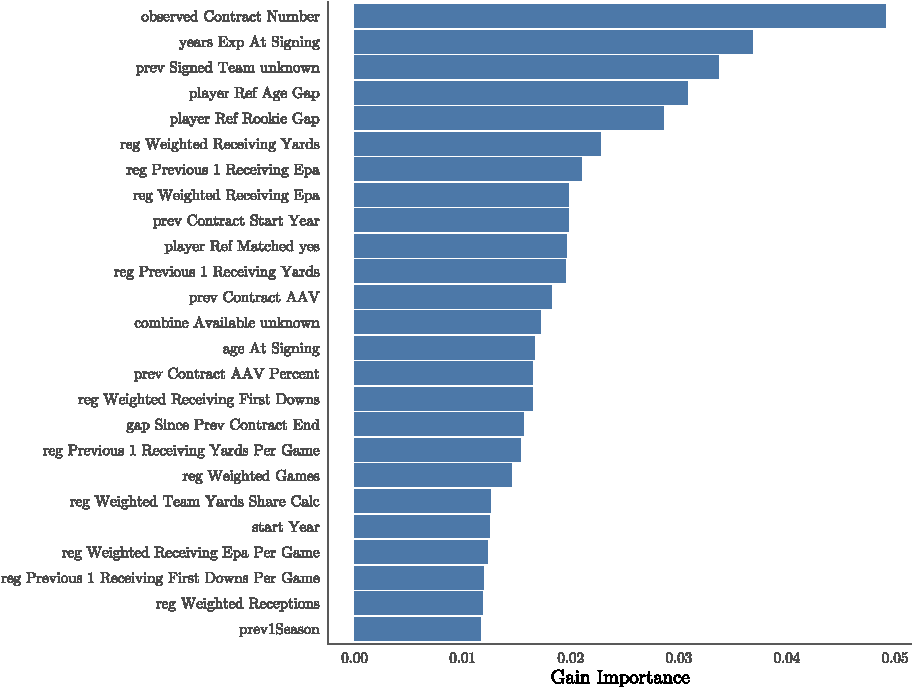
\includegraphics[width=\linewidth]{paper_files/figure-latex/term-importance-plot-1} 

}

\caption{\label{fig:term-importance} Top gain-importance features for the predictive term model.}\label{fig:term-importance-plot}
\end{figure}

Figure \ref{fig:term-importance} shows the top 25 gain-importance features for the predictive term model. Gain importance is unsigned and non-causal, but it identifies which transformed predictors most improved tree splits. Contract-history, career-stage, and match-quality features dominate, with production appearing after those market-commitment signals.

\begin{figure}[H]

{\centering 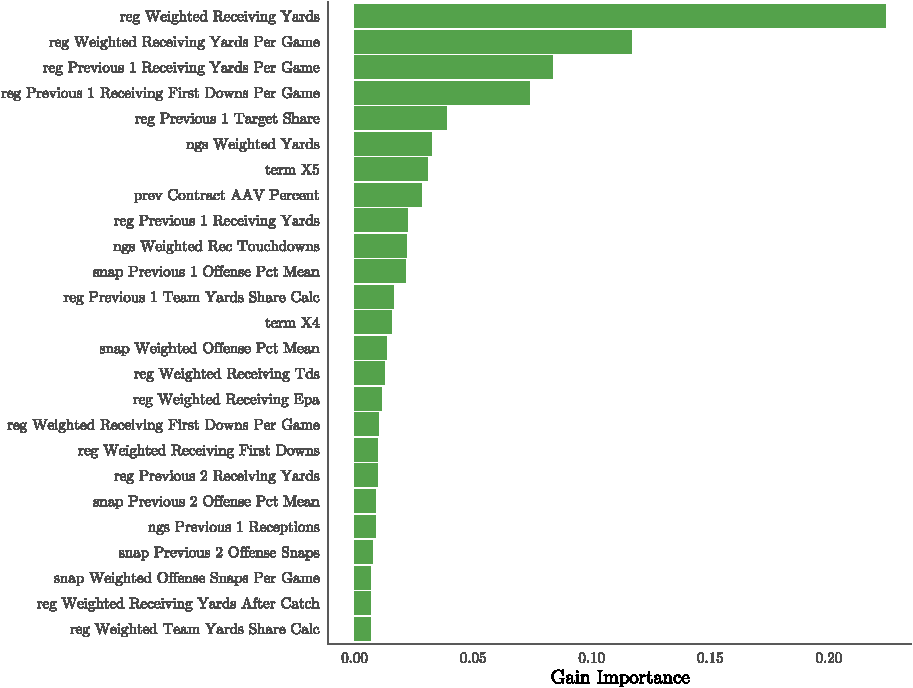
\includegraphics[width=\linewidth]{paper_files/figure-latex/aav-importance-plot-1} 

}

\caption{\label{fig:aav-importance} Top gain-importance features for the predictive conditional AAV\% model.}\label{fig:aav-importance-plot}
\end{figure}

Figure \ref{fig:aav-importance} gives the parallel importance view for the conditional AAV\% model. Receiving value, target share, prior market price, snap role, and term indicators drive compensation more directly than they drive term.

\begin{table}[H]
\centering
\caption{\label{tab:appendix-lasso-sparsity}\label{tab:lasso-sparsity} Class-specific sparsity in the lasso multinomial term model.}
\centering
\resizebox{\ifdim\width>\linewidth\linewidth\else\width\fi}{!}{
\fontsize{7.5}{9.5}\selectfont
\begin{tabular}[t]{cr}
\toprule
Term Class & Nonzero Coefficients\\
\midrule
1 & 67\\
2 & 45\\
3 & 22\\
4 & 9\\
5+ & 13\\
\bottomrule
\end{tabular}}
\end{table}

Table \ref{tab:lasso-sparsity} reports how many transformed predictors remain active for each term class in the lasso multinomial model. The class-specific sparsity pattern is useful because it shows that the interpretable model is not using the same number of signals for every contract length.

\begin{table}[H]
\centering
\caption{\label{tab:lasso-coefficients}\label{tab:lasso-coefs} Ten largest absolute nonzero lasso coefficients by term class.}
\centering
\resizebox{\ifdim\width>\linewidth\linewidth\else\width\fi}{!}{
\fontsize{6.1}{8.1}\selectfont
\begin{tabular}[t]{clrr}
\toprule
Term Class & Feature & Coefficient & Absolute Value\\
\midrule
1 & age At Signing & 0.319 & 0.319\\
1 & prev Contract Start Year & 0.281 & 0.281\\
1 & reg Previous 1 Games & -0.189 & 0.189\\
1 & prev Contract End Year & 0.167 & 0.167\\
1 & reg Previous 2 Games & -0.166 & 0.166\\
1 & reg Previous 1 Receiving First Downs & -0.157 & 0.157\\
1 & prior Team Same yes & -0.156 & 0.156\\
1 & reg Previous 1 Receiving Yards Per Game & -0.153 & 0.153\\
1 & ngs Weighted Percentent Share Of Intended Air Yards & -0.142 & 0.142\\
1 & market Delta Contract Count & -0.128 & 0.128\\
2 & prior Team Same unknown & 0.253 & 0.253\\
2 & gap Since Prev Contract End & -0.177 & 0.177\\
2 & reg Weighted Games & -0.162 & 0.162\\
2 & undrafted Flag yes & 0.137 & 0.137\\
2 & reg Previous 1 Receiving Yards Per Game & -0.122 & 0.122\\
2 & team Delta Carries & -0.113 & 0.113\\
2 & reg Previous 1 Receptions Per Game & -0.112 & 0.112\\
2 & team Previous 1 Games & 0.106 & 0.106\\
2 & reg Weighted Receiving Epa Per Game & -0.104 & 0.104\\
2 & market Previous 2 Median AAV & -0.094 & 0.094\\
3 & prev Signed Team unknown & 0.662 & 0.662\\
3 & player Ref Age Gap & 0.372 & 0.372\\
3 & combine Available unknown & 0.269 & 0.269\\
3 & team Weighted Receiving Air Yards & 0.161 & 0.161\\
3 & ngs Previous 1 Avg Yac Above Expectation & 0.110 & 0.110\\
3 & ngs Previous 1 Avg Cushion & 0.095 & 0.095\\
3 & prev Contract AAV & 0.037 & 0.037\\
3 & prev1Team CIN & -0.030 & 0.030\\
3 & prev1Team NYJ & -0.027 & 0.027\\
3 & prev1Team LA & 0.027 & 0.027\\
4 & prior Team Same yes & 0.183 & 0.183\\
4 & reg Previous 1 Receiving Epa & 0.169 & 0.169\\
4 & snap Weighted Offense Snaps & 0.104 & 0.104\\
4 & ngs Weighted Yards & 0.102 & 0.102\\
4 & team Previous 1 Receiving Air Yards & -0.078 & 0.078\\
4 & reg Previous 1 Rushing Yards & 0.065 & 0.065\\
4 & team Weighted Receiving Yards Per Target & 0.043 & 0.043\\
4 & combine Shuttle & 0.036 & 0.036\\
4 & ngs Weighted Yards Per Target & 0.004 & 0.004\\
5+ & start Year & -0.403 & 0.403\\
5+ & reg Weighted Team Yards Share Calc & 0.221 & 0.221\\
5+ & reg Previous 1 Receiving First Downs Per Game & 0.196 & 0.196\\
5+ & reg Previous 2 Receiving Epa Per Game & 0.140 & 0.140\\
5+ & market Previous 2 Contract Count & -0.085 & 0.085\\
5+ & reg Previous 1 Receiving Yards & 0.030 & 0.030\\
5+ & reg Previous 1 Air Yards Share & 0.019 & 0.019\\
5+ & team Delta Receiving Yards Per Target & 0.018 & 0.018\\
5+ & team Weighted Losses & -0.012 & 0.012\\
5+ & team Previous 2 Receiving Air Yards & -0.011 & 0.011\\
\bottomrule
\end{tabular}}
\end{table}

Table \ref{tab:lasso-coefs} lists the ten largest absolute nonzero lasso coefficients in each class. Coefficients are on the recipe-transformed scale, so they should be read as audit weights rather than raw-unit effects.

\begin{table}[H]
\centering
\caption{\label{tab:ridge-coefficients}\label{tab:ridge-coefs} Largest absolute coefficients in the ridge compensation model.}
\centering
\resizebox{\ifdim\width>\linewidth\linewidth\else\width\fi}{!}{
\fontsize{6.8}{8.8}\selectfont
\begin{tabular}[t]{lrr}
\toprule
Feature & Coefficient & Absolute Value\\
\midrule
term X5 & 0.004123 & 0.004123\\
term X4 & 0.002808 & 0.002808\\
term X3 & 0.001850 & 0.001850\\
prev Signed Team unknown & -0.001230 & 0.001230\\
prev Contract AAV & 0.001094 & 0.001094\\
prev Contract AAV Percent & 0.001079 & 0.001079\\
ngs Previous 2 Yards & 0.001076 & 0.001076\\
ngs Delta Avg Separation & -0.000977 & 0.000977\\
ngs Previous 1 Yards & 0.000937 & 0.000937\\
snap Previous 2 Offense Pct Mean & 0.000926 & 0.000926\\
prior Team Same yes & 0.000908 & 0.000908\\
reg Years Available & -0.000882 & 0.000882\\
reg Previous 2 Available yes & -0.000868 & 0.000868\\
reg Weighted Games & -0.000859 & 0.000859\\
reg Previous 1 Receiving Yards & 0.000828 & 0.000828\\
reg Previous 1 Receiving Yards Per Game & 0.000819 & 0.000819\\
ngs Previous 1 Avg Yac Above Expectation & 0.000814 & 0.000814\\
undrafted Flag yes & -0.000814 & 0.000814\\
reg Weighted Receiving Tds & 0.000811 & 0.000811\\
reg Previous 1 Available yes & -0.000808 & 0.000808\\
team Years Available & 0.000761 & 0.000761\\
ngs Previous 1 Receptions & 0.000756 & 0.000756\\
reg Previous 2 Receiving Tds & 0.000746 & 0.000746\\
snap Previous 2 Offense Snaps Per Game & 0.000734 & 0.000734\\
reg Previous 1 Receiving Epa & 0.000733 & 0.000733\\
\bottomrule
\end{tabular}}
\end{table}

Table \ref{tab:ridge-coefs} gives the 25 largest absolute coefficients from the ridge compensation model. Ridge keeps all transformed predictors but shrinks them, so the largest weights are the best compact summary of the linear audit model.

\subsection{Appendix D: Forecast Outputs}\label{appendix-d-forecast-outputs}

\begin{table}[H]
\centering
\caption{\label{tab:forecast-summary-table}\label{tab:forecast-summary} Market-level summary of unsigned 2026 WR projections from the predictive pair.}
\centering
\resizebox{\ifdim\width>\linewidth\linewidth\else\width\fi}{!}{
\fontsize{7.5}{9.5}\selectfont
\begin{tabular}[t]{lr}
\toprule
Quantity & Value\\
\midrule
Scored unsigned players & 163\\
Players with modal one-year term & 163\\
Mean one-year probability & 85.8\%\\
Mean multi-year probability & 14.2\%\\
Mean expected AAV & \$1.49M\\
Median expected AAV & \$1.11M\\
Maximum expected AAV & \$11.52M\\
\bottomrule
\end{tabular}}
\end{table}

Table \ref{tab:forecast-summary} summarizes the final scoring run. It is a market-level summary, not a claim that every individual contract will be one year; the probabilities still leave room for player-specific multi-year outcomes.

\begin{table}[H]
\centering
\caption{\label{tab:top-projections-table}\label{tab:top-projections} Twenty highest expected-AAV projections from the predictive model pair.}
\centering
\resizebox{\ifdim\width>\linewidth\linewidth\else\width\fi}{!}{
\fontsize{6.7}{8.7}\selectfont
\begin{tabular}[t]{lrcrrrrr}
\toprule
Player & Age & Previous Team & Expected Term & P(1 Year) & P(2+ Years) & Expected AAV & Modal AAV\\
\midrule
Deebo Samuel & 30 & WAS & 1.66 & 63.9\% & 36.1\% & \$11.52M & \$10.16M\\
Jauan Jennings & 28 & SF & 1.71 & 62.3\% & 37.7\% & \$10.48M & \$9.05M\\
Keenan Allen & 33 & LAC & 1.85 & 57.1\% & 42.9\% & \$10.31M & \$8.73M\\
Sterling Shepard & 33 & TB & 1.34 & 77.4\% & 22.6\% & \$4.59M & \$4.19M\\
DeAndre Hopkins & 33 & BAL & 1.15 & 90.4\% & 9.6\% & \$4.43M & \$4.19M\\
Adam Thielen & 35 & CAR & 1.09 & 93.7\% & 6.3\% & \$4.35M & \$4.22M\\
Josh Reynolds & 31 & NYJ & 1.05 & 96.0\% & 4.0\% & \$4.06M & \$4.01M\\
Ray-Ray McCloud & 29 & ATL & 1.13 & 90.4\% & 9.6\% & \$3.07M & \$2.90M\\
Gabriel Davis & 27 & BUF & 1.20 & 87.8\% & 12.2\% & \$2.69M & \$2.36M\\
Elijah Moore & 25 & BUF & 1.09 & 94.3\% & 5.7\% & \$2.67M & \$2.51M\\
Mike Woods & 26 & CLE & 1.13 & 89.8\% & 10.2\% & \$2.62M & \$2.52M\\
Mike Williams & 31 & LAC & 1.12 & 91.5\% & 8.5\% & \$2.54M & \$2.44M\\
D'Wayne Eskridge & 28 & MIA & 1.20 & 86.7\% & 13.3\% & \$2.46M & \$2.35M\\
Tim Patrick & 32 & DET & 1.14 & 89.4\% & 10.6\% & \$2.34M & \$2.15M\\
Erik Ezukanma & 26 & MIA & 1.18 & 85.0\% & 15.0\% & \$2.14M & \$2.07M\\
Bo Melton & 26 & GB & 1.33 & 72.3\% & 27.7\% & \$2.11M & \$2.00M\\
Marquez Callaway & 27 & LV & 1.09 & 92.7\% & 7.3\% & \$2.10M & \$2.07M\\
Zay Jones & 30 & ARI & 1.06 & 95.7\% & 4.3\% & \$1.96M & \$1.92M\\
Scotty Miller & 28 & PIT & 1.27 & 82.8\% & 17.2\% & \$1.93M & \$1.81M\\
Kristian Wilkerson & 29 & BUF & 1.05 & 95.9\% & 4.1\% & \$1.90M & \$1.88M\\
\bottomrule
\end{tabular}}
\end{table}

Table \ref{tab:top-projections} expands the main-text forecast discussion to the 20 highest expected-AAV players. Expected AAV is probability-weighted over the term distribution; modal AAV is the AAV attached to the most likely term scenario.

\begin{figure}[H]

{\centering 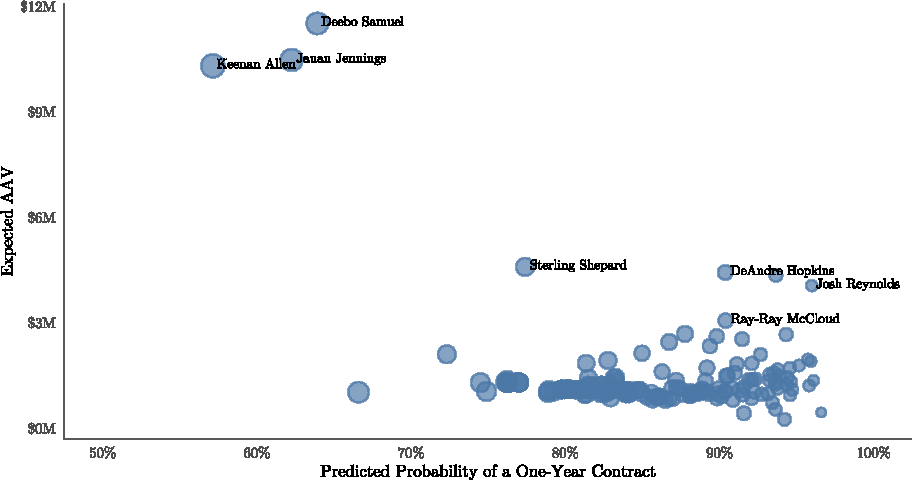
\includegraphics[width=\linewidth]{paper_files/figure-latex/market-scatter-plot-1} 

}

\caption{\label{fig:market-scatter} One-year probability versus expected AAV for unsigned 2026 wide receivers.}\label{fig:market-scatter-plot}
\end{figure}

Figure \ref{fig:market-scatter} shows the full unsigned market board. The dense cluster at high one-year probability and low AAV is the key market shape; the labeled players are high-price exceptions rather than evidence of a broad multi-year market.

\begin{figure}[H]

{\centering 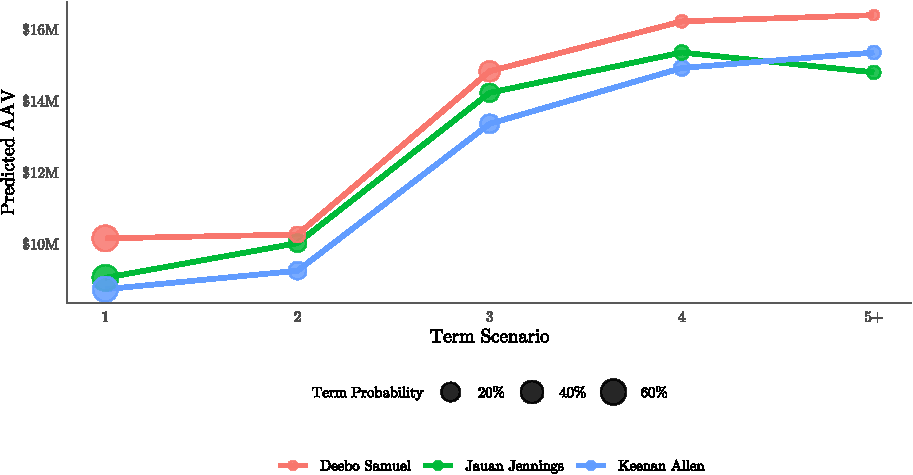
\includegraphics[width=\linewidth]{paper_files/figure-latex/scenario-paths-plot-1} 

}

\caption{\label{fig:scenario-paths} Scenario-level AAV paths for the three highest expected-AAV players. Point size is the term probability assigned by the term model.}\label{fig:scenario-paths-plot}
\end{figure}

Figure \ref{fig:scenario-paths} displays the scenario-price menu for the three highest expected-AAV players. The lines show that the price model raises AAV under longer supplied terms, but point size shows that the term model assigns most probability to the one-year point.

\newpage

\section*{References}\label{references}
\addcontentsline{toc}{section}{References}

\phantomsection\label{refs}
\begin{CSLReferences}{1}{0}
\bibitem[\citeproctext]{ref-xgboost}
Chen, Tianqi, and Carlos Guestrin. 2016. {``XGBoost: A Scalable Tree Boosting System.''} In \emph{Proceedings of the 22nd ACM SIGKDD International Conference on Knowledge Discovery and Data Mining}, 785--94. \url{https://arxiv.org/abs/1603.02754}.

\bibitem[\citeproctext]{ref-glmnet}
Friedman, Jerome, Trevor Hastie, and Robert Tibshirani. 2010. {``Regularization Paths for Generalized Linear Models via Coordinate Descent.''} \emph{Journal of Statistical Software} 33 (1): 1--22. \url{https://www.jstatsoft.org/article/view/v033i01}.

\bibitem[\citeproctext]{ref-nflreadr}
nflverse. 2026. {``Nflreadr: Download Nflverse Data.''} \url{https://nflreadr.nflverse.com/}.

\bibitem[\citeproctext]{ref-spotrac}
Spotrac. 2026. {``NFL Wide Receiver Contracts.''} \url{https://www.spotrac.com/nfl/contracts/wide-receiver/}.

\bibitem[\citeproctext]{ref-tidymodels}
tidymodels. 2026. {``Tidymodels: Easily Install and Load the Tidymodels Packages.''} \url{https://www.tidymodels.org/}.

\end{CSLReferences}

\end{document}
